
\chapter{Koncepcja biblioteki}\label{r:koncepcja}

  W tym rozdziale zostaną przedstawione główne założenia biblioteki Parallel na tle istnijących już modeli programowania równoległego, dostępnych w języku C++.

\section{Cele biblioteki}

  Tworzeniu biblioteki Parallel przyświecały jasno sprecyzowane cele, których ideą przewodnią było ułatwienie wykorzystywania obliczeń równoległych w programach.
  Wymienionym poniżej celom było podporządkowane projektowanie API i implementacja biblioteki.

\subsection{Wysoka efektywność}

  Jednym z głównych powodów stosowania zrównoleglania obliczeń jest przyspieszanie ich wykonania. Dlatego sama biblioteka do zrównoleglania powinna działać szybko.
  Niedopuszczalną byłaby sytuacja, gdyby program współbieżny wykonywał się wolniej niż jego sekwencyjny odpowiednik.
  Biblioteka Parallel będzie biblioteką ogólnego zastosowania, przy pomocy, które będzie możliwe prowadzenie dowolnych obliczeń.
  W związu z tym, nie ma możliwości zoptymalizowania biblioteki pod kątem prowadzenia pewnego typu obliczeń.
  Dlatego, oprócz szybkiego działania mechanizmów wbudowanych w bibliotekę, niezbędne jest pozwolenie programiście na podejmowanie decyzji o takim prowadzeniu obliczeń, że ich wykonanie przy użyciu biblioteki Parallel będzie efektywne.
  Kluczową rolę odgrywa odpowiedni podział zadań przez programistę (granularność obliczeń).
  
\subsection{Zwiększenie produktywności programisty}
  Problem z efektywnością programisty w przypadku pisania programów równoległych polega na tym, że takie programy są trude do pisania, stąd wymagają znacznych nakładów pracy programistów.
  Zrównoleglenie choćby niewielkiego fragmentu programu wymaga znacznie więcej czasu niż napisanie jego sekwencyjnego odpowiednika.
  Być może dlatego obliczenia równoległe wykorzystywane są wyłącznie wtedy, gdy już nie ma innego sposobu osiągnięcia niezbędnego minimum wydajności programu.
  Biblioteka Parallel celuje w zmianę tego stanu rzeczy, dzięki wprowadzeniu modelu programowania równoległego, który będzie tak intuicyjny jak programowanie sekwencyjne.
  Dzięki czemu napisanie kodu, który działa współbieżnie, będzie prawie tak samo szybkie jak kodu sekwencyjnego, co pozwoliłoby uzyskać programistom szybsze programy przy zbliżonej produktywności ich pracy.

\subsection{Czytelność kodu}

  Tym, co najbardziej utrudnia zrozumienie programów współbieżnych jest konieczność zrozumienia zależności pomiędzy odrębnymi równolegle działającymi częściami programu.
  Zazwyczaj te zależnośći dotyczą miejsc w kodzie, które są od siebie stosunkowo odległe.
  Mnogość niejawnych zależności i przeplotów wykonań programu sprawiają, że nawet pozornie proste operacje są trudne do poprawnego zaprogramowania, a przyczyny ewentualnych błędów są bardzo trudne do zidentyfikowania.
  Jednym z bardziej wymownych przykładów popierających to stwierdzenie jest problem implementacji semafora uogólnionego przy pomocy semaforów binarnych \cite{gensem}, gdzie błędne rozwiązania pojawiały się w publikacjach naukowych i nawet przez długie okresy czasu były uważane za poprawne.
  Stąd celem, który został postawiony przed biblioteką Parallel było stworzenie takiego modelu obliczeń, w którym obliczenia równoległe prowadzone byłyby w sposób czytelny.
  Oznacza to, iż miejsca wykorzystania równoległości powinny być wyraźnie widoczne i łatwe do odnalezienia, a sam zapis nie powinnien komplikować kodu.
  Najważniejsze jest to, że struktura programu napisanego przy pomocy biblioteki Parallel nie powinna istotnie różnić się od struktury programu sekwencyjnego.
  Pozwoli to na uzyskanie kodu, który będzie znacznie łatwiej zrozumieć.

\subsection{Transparencja}

  Biblioteka Parallel powinna udostępniać programiście wgląd w to, w jaki sposób oblczenia równoległe będą prowadzone.
  Dzięki temu programista będzie mógł uwzględnić podczas programowania specyfikę biblioteki.
  Między innymi będzie mógł dostosować wielkość zlecanych fragmentów obliczeń (ziarnistość obliczeń), tak aby zmaksymalizować wydajność programu.
  
% \subsection{Abstrakcja}
% 
%   Abstrakcja ukrywa niepotrzebne szczegóły implementacji przed programistą, co pozwala na zwiększenie jego produktywności.
%   Biblioteka powinna ofertować proste ogólne API, tak aby programista mógł bez 

\subsection{Ograniczenie konieczności korzystania z mechanizmów komunikacji i synchronizacji procesów równoległych}

  Projektowawnie komunikacji i synchronizacji w programach współbieżnych jest czymś, co decyduje o fakcie, że programowanie równoległe jest tak trudnym zadaniem.
  Celem biblioteki Parallel jest zdjęcie w znacznym stopniu tego obciążenia z programisty.
  Komunikacja pomiędzy różnymi wątkami wykonania będzie koordynowana przez bibliotekę.
  Biblioteka nie może wyręczyć jednak programisty we wszystkim, ochrona spójności struktur danych programu pozostanie w rękach programisty.
  
\subsection{Przenaszalność}
  
  Jest to bardzo istotna cecha biblioteki, dzięki której kod pisany przy użyciu biblioteki Parallel będzie mógł być kompilowany i wykonywany na dowolnych platformach.
  Zostanie to osiągnięte dzięki zaprogramowaniu biblioteki w pełnej zgodności z nowym standardem języka C++ (standard C++0x).
  Użycie nowego standardu jest niezbędne ze względu na zaawansowane konstrukcje językowe potrzebne do zaprogramowania biblioteki Parallel.
  Konsekwencją tego będzie niezgodność biblioteki z wcześniejszymi standardami języka C++, ale umożliwi stworzenie lepszego, bardziej czytelnego kodu biblioteki przy użyciu nowoczesnych technik programowania w C++.


\section{Prezentacja idei biblioteki Parallel}

  Niniejsza sekcja przedstawia inspirację oraz wynik końcowy pracy koncepcyjnej nad biblioteką.
  Zostaną zarysowane wysokopoziomowa architektura biblioteki oraz funkcjonowanie biblioteki z punktu widzenia programisty-użytkownika.

\subsection{Inspiracja}

  Powstanie biblioteki zostało zainspirowane biblioteką do prowadzenia obliczeń równoległych w języku Haskell, Parallel Haskell\cite{parhas}.
  Ta biblioteka pozwala w sposób bardzo intuicyjny obliczać dwa wyrażenia równolegle.
  Oto przykład funkcji obliczającej w sposób równoległy n-tą liczbę Fibonacciego:
  \begin{lstlisting}[language=Haskell]
    import Control.Parallel

    nfib :: Int -> Int
    nfib n | n <= 1 = 1
       | otherwise = par n1 (seq n2 (n1 + n2))
                     where n1 = nfib (n-1)
                           n2 = nfib (n-2)
  \end{lstlisting}
  
  Analogiczny program sekwencyjny wyglądałby następująco:
  \begin{lstlisting}[language=Haskell]
    import Control.Parallel

    nfib :: Int -> Int
    nfib n | n <= 1 = 1
       | otherwise = (n1 + n2)
                     where n1 = nfib (n-1)
                           n2 = nfib (n-2)
  \end{lstlisting}
  
  W Haskellu funkcja \verb|par| wskazuje, że wyliczenie dwóch wyrażeń może odbyć się równolegle i w czasie wykonania podejmowana jest decyzja o sposobie wyliczenia.
  Obliczenia odbywają się równolegle, gdy jest to bardziej efektywne od wykonania sekwencyjnego.
  Ta konstrukcja pokazuje z jak zadziwiającą prostotą można pisać programy równoległe.
  W Haskellu wystarczy dodać jedno słowo, aby oznaczyć wyrażenie jako przeznaczone do zrównoleglenia.
  Taka była pierwotna inspiracja dla zbudowania biblioteki Parallel.
  Przekazanie wyrażenia do odpowiedniej funkcji powinno poskutkować jego zrównolegleniem.
  
\subsection{Zlecanie obliczeń}\label{ss:zlecanie}

%  UWAGA!!! We wszystkich przedstawionych poniżej fragmentach kodu przyjęto, że zostały napisane z deklaracją \verb|using parallel;|.\\

  Zlecanie równoległego wykonania obliczeń powinno jak najmniej ingerować w sekwencyjny kod programu dla zachowania jego intuicyjności.
  (Dla wyjaśnienia dodam, że nie twierdzę, iż jedynie sekwencyjny kod programu może być intuicyjny, jednak praktyka pokazuje, że zrozumienie programu, 
  który został zapisany jako kilka jednocześnie wykonywanych ciągów instrukcji jest znacznie trudniejsze od zrozumienia programu sekwencyjnego.)
  Do oznaczenia wyrażenia, które ma zostać wykonane równolegle będzie służyła funkcja \verb|eval|, przyjmująca jako argument wyrażenie do wykonania.
  Obliczenie przekazanego wyrażenia odbędzie się równolegle.
  
  Składnia wyrażeń powinna być jak najbardziej zbliżona do składni języka C++, bo to by konstruowanie wyrażeń było łatwe dla programisty.
  Idealnie byłoby, gdyby programista mógł przekazać wyrażenie w jego standardowej postaci w języku C++, czyli w następujący sposób:
  \begin{lstlisting}[numbers=none, frame=none]
    parallel::eval(fibonacci_od(40));
  \end{lstlisting}
  W tej chwili czytelnik dobrze zaznajomiony z semantyką języka C++ mógł dostrzec pewien problem do pokonania związany z przekazaniem wyrażenia do wykonania.
  W podanym przykładzie takie wyrażenie najpierw zostałoby wyliczone, ponieważ język C++ posiada gorliwą semantykę wyliczania wyrażeń, a dopiero następnie byłoby przekazane do funkcji \verb|eval|.
  Zatem funkcja eval otrzymałaby gotowy wynik i żadne równoległe obliczenia nie byłyby już potrzebne.
  Takiej sytuacji należy uniknąć poprzez zaprojektowanie specjalnego sposobu przekazywania wyrażeń do funkcji \feval.
  Zabieg, który należy zastosować nazywa się uleniwieniem wyrażenia i polega na odroczeniu obliczenia wartości wyrażenia do momentu, gdy ta wartość będzie potrzebna.
  Wyrażenie leniwe nie jest wyliczane w miejscu pojawienia się.
  Dzięki zastosowaniu takiem metody wyrażenie, które ma być wyliczone równolegle pojawia się w kodzie tam, gdzie jest to najwygodniejsze, w jawnej postaci, a potem może zostać przekazane od mechanizmu ewaluacji biblioteki Parallel.
  
\subsubsection{Leniwe wyrażenia w języku C++}

  Stworzenie leniwego wyrażenia w języku C++ nie wydaje się prostym zadaniem.
  Domyśla semantyka obliczeń jest gorliwa, nie ma słów kluczowych pozwalających na dodanie leniwości, C++ nie pozwala również na rozszerzenie składni języka.
  Wskazówka do rozwiazanie problemu leniwych wyrażeń w języku C++ znajduje się w książce \textit{More C++ Idioms}\cite{idioms}, która przedstawia idiom C++ szablonu wyrażenia (z ang. Expression Template).
  Idea stworzenia szablonu wyrażenia polega na reprezentacji wyrażenia przez zbudowanie odpowiedniego drzewa typów, które jest Abstrakcyjnym Drzewem Syntaktycznym (z ang. Abstract Syntax Tree - AST) wyrażenia.
  Dokładny opis zastosowanej metody znajduje się w rozdziale poświęconym implementacji biblioteki.
  
  \subsubsection{Funkcja \texttt{eval}}\label{sss:eval}

  Jeszcze słowo w rozdziale przedstawiającym koncepcje biblioteki należy się funkcji \feval, która jest główną funkcją z API dostępnego dla programisty.
  Funkcja służy do zlecenia wykonania obliczeń równoleglych.
  W ciele funkcji znajduje się przekazanie wyrażenia w formie leniwej do mechanizmu ewaluacyjnego.
  Wartość zwracana przez funkcję powinna udostępniać możliwość sprawdzenia wyniku obliczenia.
  Przekazywanie wyników obliczeń przez bibliotekę Parallel zostało omówione w sekcji \nameref{s:koncepcja_wynik}.
  
\subsection{Wykonanie zadań}

  W tej podsekcji zostanie omówiony mechanizm wyliczania wyrażeń w bibliotece Parallel po przekazaniu ich do funkcji \texttt{eval}.
  Jest to serce biblioteki, dzięki któremu biblioteka potrafi pełnić swoje funkcje.
  
  \subsubsection{Działanie mechanizmu ewaluacji}
  
  Ewaluacja wyrażeń przekazanych do obliczenia będzie odbywała się zgodnie z wzorcem producent-konsument.
  Producentem wyrażeń będzie kod programu korzystającego z biblioteki Parallel i przekazujący wyrażenia przy pomocy funkcji \texttt{eval}.
  Natomiast konsumentem będą wątki-pracownicy biblioteki Parallel, których jedynym zadaniem będzie oczekiwanie na zadania (wyrażenia do ewaluacji) i ich wykonywanie.
  Ze względu na efektywność wykorzystany zostanie wzorzec puli wątków (thread pool opisany w \cite{threadpool}).
  Zatem wątek nie będzie tworzony dla wykonania każdego zadania, a będzie istniała grupa wątkół dedykowanych do wykonywania obliczeń, która będzie zaalokowana w programie tak długo jak program będzie korzystał z biblioteki Parallel.
  O liczbie wątków będzie decydował użytkownik, gdyż ich liczba może mieć znaczący wpływ na wydajność programu, a nie istnieje optymalna liczba wątków dla każdego rodzaju zastosowania biblioteki Parallel.
  Standardowo w tym modelu wyrażenia będą trafiały do kolejki zadań, w której będą oczekiwały na wyliczenie.
  
  Może się zdarzyć, że wyrażenie nie zostanie wyliczone do momentu gdy będzie potrzebne w programie, który przekazał je do obliczenia.
  W tej sytuacji biblioteka Parallel reaguje w takie sposób, by nie blokować programu bez przyczyny.
  Program dotarłby do takiego miejsca, że potrzebuje wyliczonego wyrażenia przekazanego do Parallel, a nie zostało jeszcze wykonane, program musiałby oczekiwać na wykonanie obliczeń.
  Skoro program nie ma nic innego do wykonania to wątek programu sam może wyliczyć wyrażenie, odpowiednio informując bibliotekę Parallel, aby wyrażenie nie zostało wykonane kilkakrotnie, 
  gdyż nierozsądne byłoby narzucanie ograniczenia nakazującego, żeby wyrażenia przekazywane do biblioteki Parallel były idempotentne.
  Całością procesu alternatywnego wyliczania obliczenia przez wątek programu powinna zarządzać biblioteka, tak aby nie było to zauważalne dla programisty.
  
  Jednym z rozszerzeń mechanizmu ewaluacji mogłoby być dodanie automatycznego dostosowywania liczby wątków w puli do intensywności prowadzonych obliczeń.
  W pierwszej wersji biblioteki nie przewidziano w projekcie takiej funkcjonalności.
  
  W bibliotece nie występuje problem balansowania obciążenia różnych wątków, gdyż wszystkie wątki należące do puli są identycznie i dzięki wykorzystaniu wspólnej kolejki zadań, obciążenie jest równoważone samoczynnie.
  Wątek kończąc pracę nad jednym zadaniem sięga do kolejki po następne.
  
\subsubsection{Ograniczenia mechanizmu ewaluacji}

  W związku ze sposobem przekazywania wyrażeń do obliczenia, możliwości projektowania mechanizmu ewaluacyji były dość poważnie ograniczone.
  W ogólności moglibyśmy wyobrazić sobie sytuację, w której wyrażenie z programu działającego na jednym komputerze byłoby przekazywane do wyliczenia do innych programów lub nawet do innych komputerów, w celu większego rozproszenia i jeszcze lepszego zrównoleglenia wykonania programu.
  W przypadku biblioteki parallel wystąpiło kilka ograniczeń, które uniemożliwiły zaprojektowanie ogólniejszego mechanizmu obliczeń.
  
  Migracja kodu (taka jak zostałą opisana w książce \cite{dissys}) nie jest wspierana przez język C++, ponieważ kod kompilowany jest do natywnego kodu maszynowego, a nie kodu pośredniego.
  Nie ma możliwości zserializowania fragmentu obliczeń i przesłania do wykonania na innym komputerze, o nieznanej architekturze.
  W przeciwieństwie do języka C++ to jest wykonalne w języku Java.
  
  Alternatywą dla wsparcia języka dla migracji kodu jest rozszerzenie biblioteki o narzędzia automatycznie generujące kod dla klienta (programu zlecającego obliczenia) i serwera (programu wykonującego obliczenia).
  To już zaczyna przypominać mechanizm RPC i rodzi szereg innych problemów również opisanych w \cite{dissys}.
  Implementacja takiego modelu prowadzenia obliczeń w bibliotece Parallel wykraczałaby poza ramy nakreślonej pracy oraz mogłaby ograniczyć użyteczność biblioteki ze względnu na bardziej skomplikowany proces programowania i kompilacji.
  
  Kolejne z ograniczeń jest związane z obecnością w wyrażeniu przekazywanym do obliczenia wartości typu referencje lub wskaźniki, które są ściśle zależne od przestrzeni adresowej programu. 
  Przesłanie ich nawet do innego programu na tym samym komputerze wymagałoby wykorzystania specjalnego mechanizmu, gdyż proste przekazanie wartości tego typu powodowałoby błędy w dostępie do pamięci.
  Obejście tego problemu oferuje mechanizm pamięci współdzielonej, ale powoduje znaczny narzut związany z dostępnem do tego rodzaju pamięci.
 
  Wymienione powyżej ograniczenia uzasadniają podjęcie decyzji o przyjęcie dla biblioteki Parallel modelu obliczania wyrażeń opartego o wątki działające w ramach programu zlecającego obliczenia.
  
% \subsubsection{Mechanizmy synchronizacji}
% 
%   Dla poprawności działania biblioteki niezbędne było zaimplementowanie mechanizmu synchronizacji wątków-pracowników oraz kodu programu. 
%   Przede wszystkim, ochrony przed wspólbieżnym dostępem wymaga kolejka zadań, na której będę jednocześnie operowały wszystkie wątki z puli, w celu pobierania obliczeń do wykonania, oraz kod programu użytkownika, w celu dodania wyrażenia do obliczenia.
%   Aby zapewnić tym operacjom bezpieczeńśtwo wystarczy dostęp do kolejki zadań otoczyć sekcją krytyczną, w której będzie mógł przebywać tylko jeden program.
%   
%   Ponadto, należy chronić zadania przed podwójnym wyliczeniem, przez wątek programu oraz przez wątek-pracownika biblioteki Parallel.
%   Mogłoby to mieć miejsce, gdyż jak zostało to nadmienione powyżej, kod programu użytkownika zamiast czekać aż wyrażenie się wyliczy, może sam to zrobić, jeśli biblioteka nie rozpoczęła jeszcze ewaluacji danego wyrażenia.
%   Stąd kod użytkownika, gdy rozpocznie samodzielne wyliczenie wyrażenia oznacza je jako wykonane.
%   
%   Biblioteka nie może przewidzieć zależności w kodzie programu, dlatego ochrona danych, na których dokonywane są obliczenia pozostanie w rękach programisty.
%   Parallel nie narzuca żadnych ograniczeń, co do korzystania w kodzie zrównoleglanych wyrażeń instrukcji dostępu do struktur danych, z których korzysta wiele wątków jednoczesnie.
%   W tej sytuacji programista musi zadbać o odpowiednie umieszczenie sekcji krytycznych w kodzie obliczanych wyrażeń, tak aby program był bezpieczny i żywotny.
  
\subsection{Sposób przekazywania wyniku}\label{s:koncepcja_wynik}

  Kod korzystający z biblioteki Parallel powinien wyglądać naturalnie.
  Skoro do funkcji \texttt{eval} przekazujemy wyrażenie, to naturalnym oczekiwaniem jest to, że w wyniku ewaluacji otrzymamy wartość tego wyrażenia.
  Problem leży w tym, że w momencie powrotu z funkcji \texttt{eval} będzie znany jedynie typ wyrażenia, a nie jego wartość.
  Wartość zostanie obliczona później przez mechanizm ewaluacji biblioteki Parallel.
  Wynika stąd potrzeba wprowadzenie klasy obudowującej wartość zwracaną, uchwytu do wyniku, nazwijmy go wartością odroczoną (z ang. deferred value).
  Aby wartość odroczona ściśle odpowiadała typowi wynikowemu wyrażenia, będzie ona szablonem typu parametryzowanym typem wynikowym wyrażenia.
  Dzięki temu, że znany był typ zwracany, możliwe jest takie zaprojektowanie klasy wartości odroczonej, że przypomina w swoim zachowaniu typ wynikowy wyrażenia.
  
  Wartości odroczonej można używać prawie zamiennie z typem, który obudowuje.
  To dzięki temu, że jest dostępna niejawna konwersja do obudowywanego typu, a zastosowanie operatorów będzie dawało identyczny wynik.
  W momencie, gdy wartość wyrażenia będzie niezbędna nastąpi wymuszenie ewaluacji, jeśli wartość nie została jeszcze wyliczona, i pobranie wyniku.
  Przykładem takiej sytuacji jest przypisanie wartości odroczonej na zmienną o typie wartości obudowywanej.
  Odbędzie się wtedy niejawna konwersja, do której będzie potrzebna rzeczywista wartość wyrażenia.
  
\subsubsection{Obsługa sytuacji wyjątkowych}
  Należy również przyjrzeć się sytuacji, w której w czasie obliczania wyrażenia wystąpi błąd, zasygnalizowany przez rzucenie wyjątku.
  Biblioteka Parallel powinna wspierać obsługę takiej sytuacji w kodzie.
  Aby reakcja ze strony programisty była możliwa wyjątek musi zostać złapany i zasygnalizowany programiście.
  Przepuszczenie wyjątku przez bibliotekę skutkowałoby natychmiastowym błędnym zakończeniem programu, 
  gdyż programista nie miałby żadnej możliwości złapania wyjątku, gdyż wyjątek ten pochodziłby z kodu biblioteki Parallel wykonywanym w innym wątku.
  Biblioteka nie powinna również tłumić wszystkich wyjątków, gdyż programista nie wiedziałby wtedy co się dzieje w programie, a wartość przypisana na wartość odroczoną byłaby niezdefinowana.
  
  Nasuwa się zatem rozwiązanie, w którym biblioteka wyłapywałaby wyjątki wywołane w obliczanych wyrażeniach, ale przekazywane byłyby one do wątku głównego programu.
  Może to nastąpić jedynie za pośrednictwem wartości odroczonej, ponieważ powrót z funkcji \feval następuje zazwyczaj przed rozpoczęciem obliczania wyrażenia.
  Wartość odroczona ma ustalony typ, więc wartość odroczona nie może zwrócić wyjątku.
  Jednakże, to co może zostać wykonane to ponowne rzucenie wyłapanego i przekazanego do wartości odroczonej wyjątku przy próbie pobrania wyliczonej wartości.
  Wtedy wyjątek powstały w obliczeniach byłby przekazywany do kodu głównego wątku i programista miałby możliwość jego obsługi w dobrze zdefinowanym miejscu.
  
% \subsubsection{Metody klasy reprezentującej uchwyt do wyniku}
% 
%   Interfejs publiczny klasy reprezentującej uchwyt do wyniku będzie zawierał metody:
% \begin{itemize}
%  \item pobrania wartości,
%  \item sprawdzenia czy wartość została już wyliczona,
%  \item operator konwersji do typu wyniku wyrażenia
% \end{itemize}
% 
% \paragraph{Operatory}~\\
%   Ponadto w interfejsie klasy obudowującej wynik będą znajdowały się wszystkie operatory, które mają sens dla typu obudowywanego.
%   Oczywiście ze względu na  ograniczenia języka niemożliwe jest zdefinowanie operatorów, których przeładowywanie jest zabronione, takich jak \verb|.| oraz \verb|.*|.
%   
%   Możliwa jest taka sytuacja, w której wykorzystanie wartości odroczonej w wyrażeniu nie będzie wymuszało natychmiastowego wyliczenia wartości odroczonej.
%   Weźmy jako przykład nastepującą instrukcję:
% \begin{verbatim}
%   auto c = odroczony_int + 42;
% \end{verbatim}
%   Czy musimy znać wartość odroczony\_int, aby przypisać odpowiednią wartość na zmienną c?
%   To zależy w tym przypadku od implementacji operatora \verb|+|.
%   Jeśli operator dodawania będzie tak zaprojektowany, że dodanie wartości odroczonej sparametryzowanej typem int oraz liczby całkowitej zwraca inta, to oczywiście wartość odroczona musi być znana.
%   Natomiast dzięki temu, że przytoczona w przykładzie instrukcja zawiera pewną dowolność w postaci automatycznego typowania zmiennej c, to nic nie stoi na przeszkodzie, żeby c było również wartością odroczoną.
%   I taka decyzja projektowa została podjęta w bibliotece Parallel.
%   Operatory będą zwracać wartość typu wartość odroczona, aby prowadzić obliczenia w taki sposób, że wymuszenie obliczenia wartości odroczonej było odłożone najpóźniej jak to możliwe.
%   Wartość odroczna zwracana przez operatory, będzie zawierała leniwe wyrażenie podobne do tego, które jest przekazywane funkcji \verb|eval|.
%   W momencie wymuszenia wyliczenia takiej wartości odroczonej to leniwe wyrażenie zostanie wyliczone.
%   Pozwoli to na lepsze zrównoleglenie obliczeń, ponieważ umożliwie przeprowadzenie większej liczby obliczeń przez wątki-pracowników z biblioteki Parallel.
%   
%\subsubsection{Wpływ sposobu przekazywania wyniku na cele biblioteki Parallel}

\subsection{Schemat interakcji kodu programu z biblioteką Parallel}

  Podsumowania opisu idei biblioteki Parallel dokonam poprzez opisanie pokrótce tego jak kod aplikacji pisany przez programistę współpracuje z kodem biblioteki Parallel.
  Schematycznie ilustruje to poniższy diagram.
\begin{figure}[h!]
 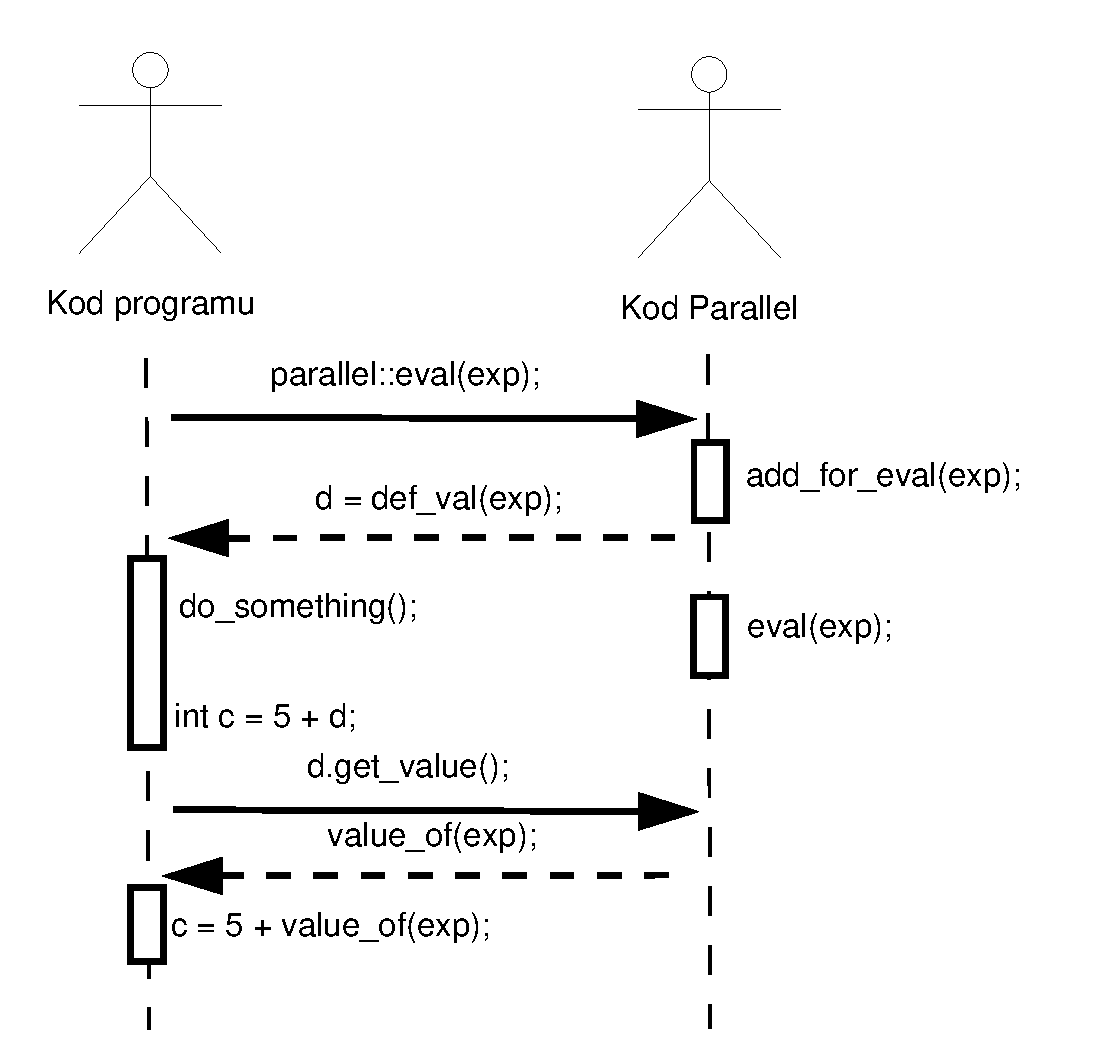
\includegraphics[width=\textwidth]{interaction.eps}
 \caption{Schemat interakcji z biblioteką Parallel}
\end{figure}

  Schemat pokazuje jak w pierwszej kolejności kod programu wywołuje funkcję \feval, która służy do zlecenia obliczenia równoległego wyrażenia.
  Następnie sterowanie przechodzi do ciała funkcji \feval, czyli do kodu biblioteki Parallel.
  Funkca \feval tworzy niezbędne struktury danych oraz dodaje wyrażenie \verb|exp| do wyrażeń czekających na wyliczenie.
  Potem następuje powrót z funkcji \feval ze zwróceniem wartości odroczonej \verb|d| i na jakiś czas kod programu i biblioteki Parallel zaprzestają komunikacji.
  Kod programu wykonuje własne instrukcje, a kod Parallel wykonuje własne zadania, między innymi wyliczając wyrażenia, które zostały wskazane do wyliczenia równoległego.
  Takie wyliczenie zachodzi w pewnym momencie w czasie równiez dla wyrażenia \verb|exp|.
  
  Gdy nadchodzi moment w kodzie programu, gdy potrzebna jest wyliczona wartość wyrażenia to następuje automatycznie próba pobrania wartości wyrażenia z wartości odroczonej \verb|d|.
  Wtedy następuje przekazanie sterowania do kodu biblioteki, który przekazuje z powrotem wyliczoną wartość wyrażenia \verb|exp|.
  Kod programu otrzymuje wartość i może dalej prowadzić swoje obliczenia.
  Tak wygląda jeden cykl skorzystania z mechanizmu zlecania wyrażeń do równoległego wyliczenia w bibliotece Parallel.
  